\chapter{Obsah přiloženého CD}
Struktura přiloženého CD
\begin{itemize}
\item \textbf{README.txt} - Textový soubor popisující obsah CD
\item \textbf{src/} - Adresář obsahující zdrojové kódy
\item \textbf{thesis/} - Adresář obsahující písemnou zprávu a její zdrojové kódy
\item \textbf{misc/} - Adresář obsahující plakát a vyhodnocení uživatelského testování
\end{itemize}

\chapter{Přiložené obrázky}
\begin{figure}[H]
	\centering
	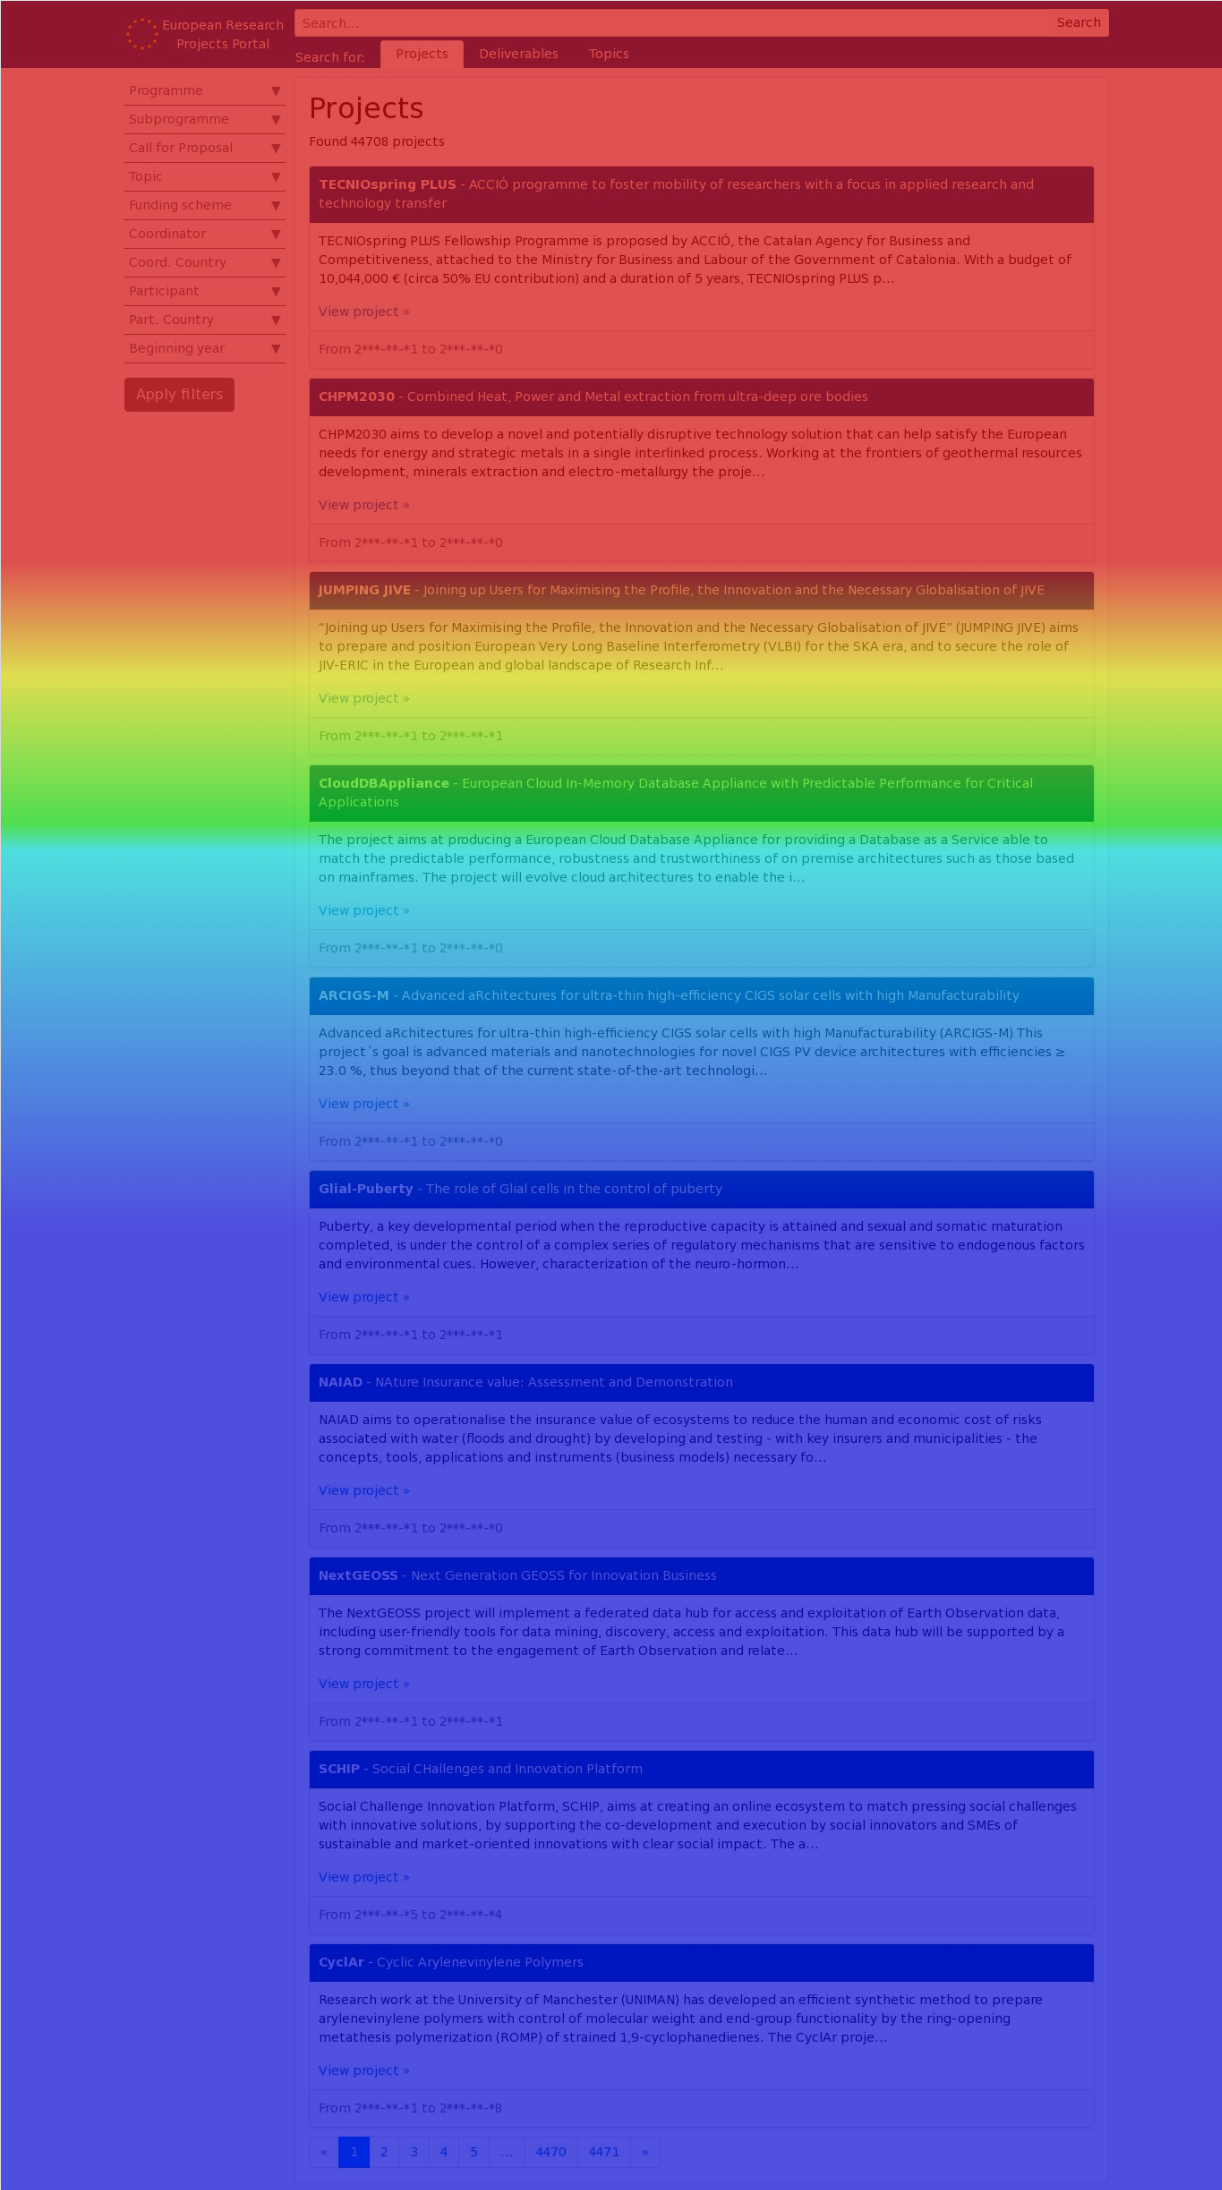
\includegraphics[height=\textheight-8cm]{obrazky-figures/heatmap-scroll.png}
	\caption{Tepelná mapa rolování uživatelů na stránce prezentující výsledky vyhledávání.}
    \label{img:heatmap-scroll}
\end{figure}